\section{Taxonomy}

\begin{figure*}[ht]
    \centering
    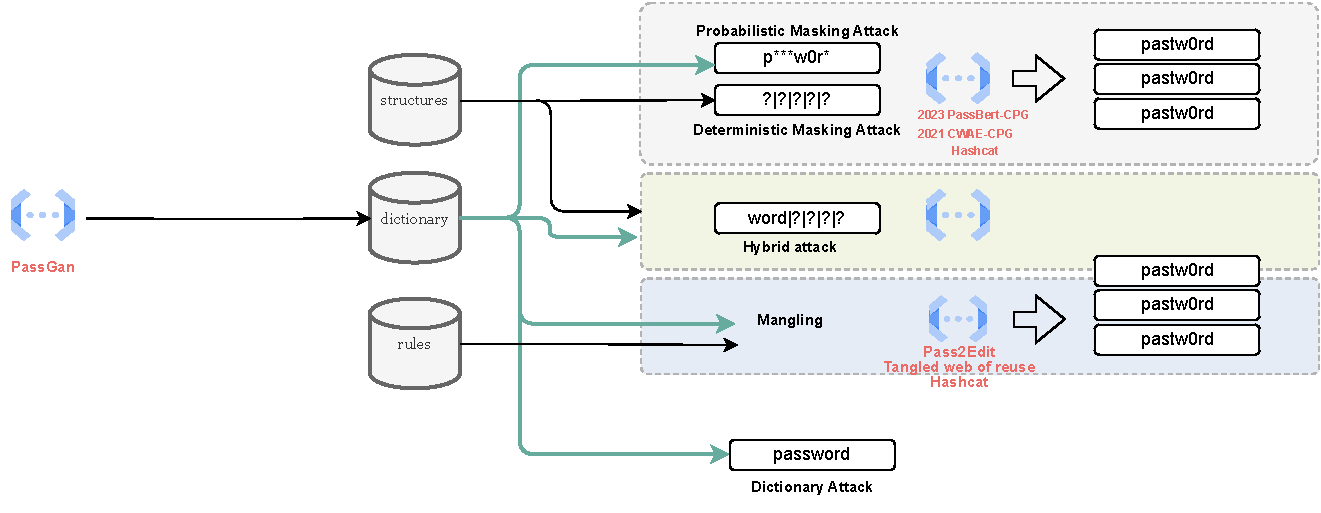
\includegraphics[scale=0.7]{figs/how_passwords/mindmap_structure2.pdf}
    \caption{Caption}
    \label{fig:enter-label}
\end{figure*}

We can compare the prior literature on password guessing using two methods: 1) comparison using implementation methodology (e.g. probabilistic vs deep learning methods); 2) method and type of attack (e.g. offline vs online attack).

Most human-chosen secrets are susceptible to pre-image attack: Given some hash value, $h$, find an input $m$ such that $\textbf{H}(m) = h$, where $\textbf{H}$ is some hash function. Consider $m$ to be the password or the memorised secret, then the argument is that it is computationally feasible to guess $m$. So, memorable secrets are not pre-image resistant. This chapter analyses the methods used to calculate the pre-image. The methods of attacks mentioned here are those that specifically target the weakness of the password--their guessability. So, it is usually the attacker v.s. a hash in two scenarios: 1) the attacker has the hash and is not limited to the number of guesses it can make; 2) the attacker does not have the hash (online attack) and is rate limited to the number of guesses. We can add two more scenarios: 1) the attacker knows the victim or has useful information about them; 2) the other attacker does not know the victim (e.g. trawlling attack). Figure \ref{fig:attack-types} demonstrates these scenarios visually in a matrix.

\begin{figure}[h]
    \centering
    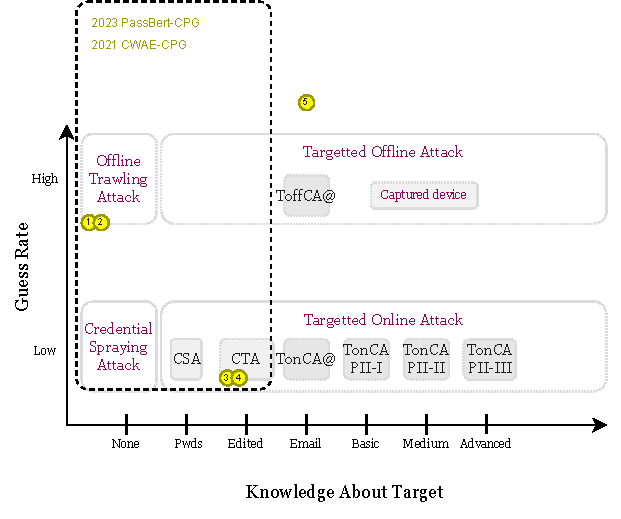
\includegraphics[scale=0.8]{figs/how_passwords/mindmap_structure.pdf}
    \caption{Caption}
    \label{fig:enter-label}
\end{figure}

\begin{figure}[h]
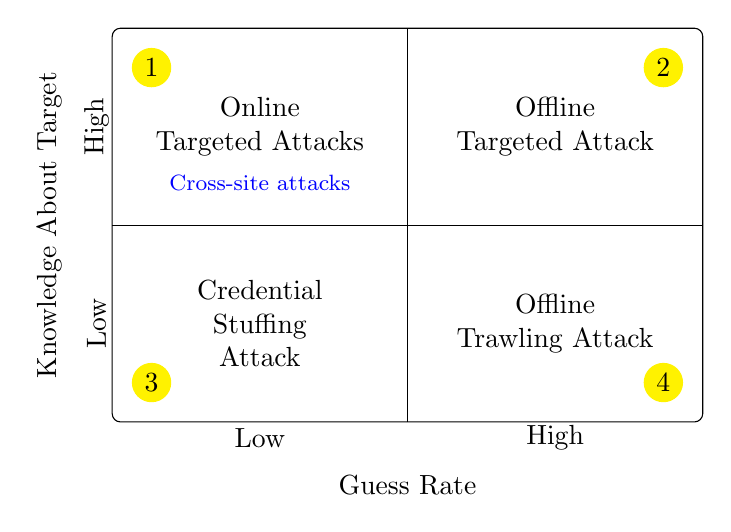
\begin{tikzpicture}
    % Variables for the grid size
    \def\gridwidth{7.5}
    \def\gridheight{5}

    % Draw the main grid
    \draw[rounded corners=3pt] (0,0) rectangle (\gridwidth,\gridheight);
    
    % Draw the dividing lines
    \draw (\gridwidth/2,0) -- (\gridwidth/2,\gridheight);
    \draw (0,\gridheight/2) -- (\gridwidth,\gridheight/2);
    
    % Labels for the attack types
    \node[align=center] (box1) at (\gridwidth/4,3*\gridheight/4) {Online\\Targeted Attacks};
    \node[align=center] at (3*\gridwidth/4,3*\gridheight/4) {Offline\\Targeted Attack};
    \node[align=center] at (\gridwidth/4,\gridheight/4) {Credential\\Stuffing\\Attack};
    \node[align=center] at (3*\gridwidth/4,\gridheight/4) {Offline\\Trawling Attack};

    \node[below, text=blue, font=\footnotesize] at (box1.south) {Cross-site attacks};
    
    % Labels for the axes
    \node[align=center] at (\gridwidth/2,-0.8) {Guess Rate};
    \node[align=center, rotate=90] at (-0.8,\gridheight/2) {Knowledge About Target};
    
    % Axis numbers
    \node[align=center] at (\gridwidth/4,-0.2) {Low};
    \node[align=center] at (3*\gridwidth/4,-0.2) {High};
    \node[align=center, rotate=90] at (-0.2,3*\gridheight/4) {High};
    \node[align=center, rotate=90] at (-0.2,\gridheight/4) {Low};


    % Circles with numbers
    % Upper left
    \node[circle,fill=yellow,inner sep=0pt,minimum size=0.5cm] at (0.5,\gridheight-0.5) {1};
    % Upper right
    \node[circle,fill=yellow,inner sep=0pt,minimum size=0.5cm] at (\gridwidth-0.5,\gridheight-0.5) {2};
    % Lower left
    \node[circle,fill=yellow,inner sep=0pt,minimum size=0.5cm] at (0.5,0.5) {3};
    % Lower right
    \node[circle,fill=yellow,inner sep=0pt,minimum size=0.5cm] at (\gridwidth-0.5,0.5) {4};

\end{tikzpicture}
\caption{Categories of attacks based on the attack rate (available to the attacker) on the horizontal axis and the amount of knowledge the attacker has about the target on the vertical axis. High attack rate signifies that the attacker has access to the target's hash. A low attack rate means that the attacker is trying to attack a hash through a website service that is rate limited.}
\label{fig:attack-types}
\end{figure}

\subsection{Models}

A guessing attack can either be completely generative or an edit function. Masking (normal and hybrid) and mangling attacks are can be described as edit functions, as they are taking a password or a structure and editing it.

\paragraph

\subsection{Context of Attack}
\paragraph*{Offline attacks}


\paragraph*{Cross-site attacks}
\begin{enumerate}
\item
  \textbf{Cross-site password attack.} Given two datasets with the same
  set of unique users but different passwords, e.g.Rockyou and
  000webhost, how many of the 000webhost passwords can I guess if I use
  the respective user's password from the Rockyou dataset?
  \item \textbf{Basic cross-site PII attack}. This attack is similar to the
    cross-site password attack but now we use more information to guess
    the password. Basic information such as name, date of birth, email,
    and other information that might be typically in a breached dataset.
  \item \textbf{Advanced cross-site PII attack}. This attack will utilise
    other information about the user in order to guess the password. For
    example information gathered from social media platforms.
\end{enumerate}

%\begin{Shaded}
%\begin{Highlighting}[]
%\NormalTok{rockyou\_data }\OperatorTok{=}\NormalTok{ \{}\StringTok{\textquotesingle{}bob@gmail.com\textquotesingle{}}\NormalTok{: }\StringTok{\textquotesingle{}password0!\textquotesingle{}}\NormalTok{, ...\}}
%\NormalTok{webhost\_data }\OperatorTok{=}\NormalTok{ \{}\StringTok{\textquotesingle{}bob@gmail.com\textquotesingle{}}\NormalTok{: }\StringTok{\textquotesingle{}p4ssword!0\textquotesingle{}}\NormalTok{, ...\}}
%
%\NormalTok{right\_guesses }\OperatorTok{=} \DecValTok{0}
%\ControlFlowTok{for}\NormalTok{ email, password }\KeywordTok{in}\NormalTok{ rockyou\_data:}
%\NormalTok{    guessed }\OperatorTok{=}\NormalTok{ guess\_password(prev\_pwd: password, iterations: }\DecValTok{100}\NormalTok{)}
%    \ControlFlowTok{if}\NormalTok{ guessed:}
%\NormalTok{        right\_guesses }\OperatorTok{+=} \DecValTok{1}
%        
%\NormalTok{percentage\_guessed\_right }\OperatorTok{=}\NormalTok{ (right\_guesses }\OperatorTok{/} \BuiltInTok{len}\NormalTok{(webhost\_data)) }\OperatorTok{*} \DecValTok{100}
%\end{Highlighting}
%\end{Shaded}


\hypertarget{evaluation-criteria}{%
\subsection{Evaluation criteria}\label{evaluation-criteria}}

\begin{itemize}
\item
  Guessing performance
\item
  Running time
\item
  Generation capacity
\item
  Duplicate rate
\item
  Model Size
\item
  Training time
\end{itemize}

\hypertarget{future-work}{%
\subsection{Future work}\label{future-work}}

\begin{itemize}
\item
  Real world attackers seldom use the techniques offered by Academia.
  The Hashat write up 2023, used a PCFG method. The work in
  {[}@pasquiniReducingBiasModeling2021{]} (Pasquini et al.~2021) argue
  that real world attackers use more pragmatic methods such as
  dictionary-based attacks. Their argument is that domani-knowledge is
  requried. So they develop new dictionary-based attacks:
  \textbf{adaptive mangling ruels attack} and \textbf{dynamic guessing
  strategies}.

  \begin{itemize}
  \item
    ``dictionary attacks describe password distributions by factorizing
    guesses into two main components---a dictionary word w and a
    transformation rule r. Here, the word w acts as a semantic base,
    whereas r is a syn- tactic transformation that aims at providing a
    suitable guess through the manipulation of w.''
  \item
    Dynamic dictionary attack

    \begin{itemize}
    \item
      THe authors argue that distribution of passwords could differ
      because of language, community interests and imposed policies.
    \item
      dynamic attacker is an adversary who changes his guessing strategy
      according to the attack's success rate
    \item
      we dynamically augment the dictionary during the attack using the
      guessed passwords.
    \end{itemize}
  \item
    The paper doesn't go into the details of the hits that worked and
    what could be done to improve it more.
  \end{itemize}
\end{itemize}


\hypertarget{offline-attack}{%
\subsection{Offline Attack}\label{offline-attack}}

\begin{table*}
\caption{Trawling attacks}
\begin{tabularx}{\textwidth}{clp{3cm}p{3cm}cc}
\toprule
Year & Model & Data & Comparison & Method & Code \\
\midrule
2023 & RFGuess & Rockyou
000webhost & FLA
PCFG
Markov & Random Forest Trees & Link \\
2023 & PassBERT-CPG & Rockyou
000webhost
Neopets
Cit0day
Rockyou-2021 & Hashcat (rule-based)
ADaMs
Vanilla BERT & Transformer & N/A \\
2022 & G-pass & & & GAN & N/A \\
2022 & STAT22 & & Markov
PCFG
Hashcat
JtR & & N/A \\
2022 & OMECDN & & OMEN
PassGAN & Markov & N/A \\
2022 & GNPassGAN & Rockyou
phpbb & PassGAN & GAN & Link \\
2021 & CPG21 & & PassGAN & GAN & Link \\
2021 & AdaMs & 4iQ & Hashcat & ANN & Link \\
2019 & PassGAN & Rockyou
LinkedIn & Markov
Hashcat
PCFG
FLA
JtR & GAN & Link \\
2016 & FLA & & PCFG
Markov
JtR
Hashcat & RNN & Link \\
2009 & PCFG & & & & Link \\
2005 & Markov & & & & \\
N/A & Hashcat & N/A & N/A & N/A & N/A \\
\bottomrule
\end{tabularx}
\end{table*}

Offline attack assumes that we are not limited to the number of guesses
we can make and therefore we have the password hash to attack. For
example, a leaked database belonging to eHarmony site has 1.5million md5
hashes but no cleartext. A clear tool in this category is Hashcat.

Dictionary attack uses a large list of generated passwords to guess and
crack a hashed password. Trawling attack is a type of password-guessing
attack where a large combination of words are used to match the target
password with. In the literature the aim of trawling attack is to create
a wordlist. In this section we will do a review of the

\textbf{Markov n-gram} \cite{narayanan_fast_2005}

\textbf{Probabilistic context-free grammar (PCFG)} \cite{weir_password_2009}

\textbf{RFGuess} \cite{wang_password_2023} (2023) uses Random Forest
trees to generate passwords. The authors have falsely called this trawlling attack, the two algorithms sit between \textit{Credential Stuffing Attack} and \textit{Online Targeted Attack}. The authors claim that is similar to the
Markov 7-gram model without much comparison to the Markov 7-gram models
in the results section. They compare the model to PCFG, Markov and FLA.
Experiment scenarios are split between different sites (cross-sites) and
inter-site, where they use a portion of the leaked password set to the
training and the remaining portion for testing. RFGuess uses the Rockyou
and 000webhost dataset for the trawling attack. The results are
inconclusive in our opinion. With a lack of tabular data it is difficult
to judge the differences in the models. The different graphs show
RFGuess performing similar to worse than its counterparts. The claim
that \emph{`RFGuess outperforms all its counterparst in intra-site
guessing scenarios'} can not be seen in the results. Lastly, the authors
falsely claim that RFGuess is suitable for online password guessing
scenarios. The results (in Fig 6 and 7 in their paper) invalidates this
statement. Their claim that online guessing is unavoidable and its
success is rather high is also false. Majority of websites implement
rate limiting in their authentication systems. In summary, the use of
Random Forest Trees for trawling attack is inconclusive from this paper
and the results are deemed to be worse than their counterparts.

\textbf{PassBERT} \cite{xu_improving_2023} introduces
three distinct attack methodologies: Conditional Password Guessing
(CPG), Targeted Password Guessing (TPG), and Adaptive Rule-based
Password Guessing (ARPG). This study focuses primarily on the
non-targeted trawling attack, namely CPG. The data pre-processing phase
involves the exclusion of hashed passwords, the elimination of non-ASCII
character passwords, and the removal of passwords exceeding 32
characters in length. Passwords undergo tokenization at the character
level, incorporating the {[}CLS{]} and {[}SEP{]} tokens to signify the
commencement and termination of sequences, respectively. The model's
pre-training employs the Rockyou-2021 dataset, utilizing a random
sampling of 60 million entries. On average, PassBERT demonstrates a
password generation rate of 4.54 passwords per second. A comparative
analysis is conducted with the Context Wasserstein Autoencoder (CWAE) as
documented in Pasquini et al.~(2021)  \cite{pasquini_improving_2021}. Notably, the referencing
of this model appears to be erroneous. The rationale provided by the
authors for selecting CWAE over Pass2path (Pal et al., 2019) \cite{pal_beyond_2019} and ADaMs (Pasquini et al.,
2021) \cite{pasquini_reducing_2021} is predicated on CWAE's
superior performance. The reproducibility of password guessing attacks
presents significant challenges. Efforts to contact the original authors
for access to the model and its weights proved futile, further
complicating the replication process.

\textbf{CWAE} \cite{pasquini_improving_2021} This paper
proposes using representation learning with deep generative models like
GANs and autoencoders for password guessing. The authors train these
models on leaked password datasets like RockYou to learn a latent
representation of passwords that captures semantic relationships. They
introduce two novel password guessing frameworks - Conditional Password
Guessing (CPG) which can generate biased guesses, and Dynamic Password
Guessing (DPG) which adapts the guessing strategy based on successfully
guessed passwords. CPG allows generating passwords matching arbitrary
templates or biases using the strong locality property of the latent
space. DPG leverages the weak locality to reduce the covariate shift
between train and test password distributions. The authors compare these
techniques against probabilistic guessers like OMEN, PCFG and FLA on
biased test sets created from LinkedIn data. They show CPG can
efficiently generate rare biased guesses unlike other methods. DPG
adapts and outperforms static attacks on diverse leaks like Youku and
Zomato exhibiting distribution shifts.

\begin{itemize}
\item
  \textbf{Trawling guessing} means that the attacker does not care who
  the specific target is.
\item
  Uses 13 large password datasets. 241.27 million pwds.
\item
  Compares it with PCFG, Markov, and FLA.
\item
  There are no tabular review of the data! hard to compare the models.
\item
  The improvement on other models is negligible.
\item
  Are they lacing the data with the test data? \emph{``Since the
  attacker is smart and will constantly improve her training set to make
  it as close as possible to the test set (to improve her
  success-rates), our intra-site experimental methodology just reflects
  this sit- uation''}
\end{itemize}

\hypertarget{methods}{%
\subsection{Methods}\label{methods}}

\begin{itemize}
\item
  \textbf{GAN}

  \begin{itemize}
  \item
    \textbf{\passgan}

    \begin{itemize}
    \item
      They referenced but did not compare the results with FLA?
      \href{https://github.com/brannondorsey/PassGAN}{According to this
      repo}. It is likely to underperform both the RNN and Markov-based
      approaches.
    \end{itemize}
  \item
    \textbf{CPG} (Conditional password guessing) and \textbf{DPG}
    (dynamic password guessing)
    {[}@pasquiniImprovingPasswordGuessing2021{]} are GAN models and an
    improvement on \emph{PassGAN} (preprinted in 2019 but published in
    2021?).
  \item
    \textbf{REDPACK} \cite{nam_generating_2020} 
  \item
    \textbf{AdaMs} \cite{pasquini_reducing_2021}
  \item
    \textbf{GNPassGAN} \cite{yu_gnpassgan_2022}
    \begin{itemize}
    \item
      \textbf{Comparison}: Only compares to \passgan
    \item
      \textbf{Training data}: Rockyou
    \item
      \textbf{Test data}: \phpbb and a disjoint subset of Rockyou.
    \item
      Experiments on two lengths

      \begin{itemize}
      \item
        Char10 \(p \leq 10\)
      \item
        Char812 \(8 \geq p \leq 12\)
        \[Matching Accuracy = \frac{\text{Count}( \text{set}(F G) \cap \text{set}(F T ))}{\text{Count}(\text{set}(F T ))}\]
      \end{itemize}
    \end{itemize}
  \end{itemize}
\end{itemize}

I have few criticisms of GNPassGAN \cite{yu_gnpassgan_2022}. It essentially uses Rockyou
dataset to generate another larger dictionary file. So, it creates a
dictionary file. But the size of the dictionary matters, the larger it
is the more hashes we have to create and therefore more time wasted on
cracking. \textbf{The order of the dictionary file} should matter.

\begin{itemize}
\item
  \textbf{Question}: Could we tailore the generated dictionary file to
  the site we are attacking? So that we have a smaller and focussed
  dictionary.
\end{itemize}

The generated (\(FG\)) file is then used to compare to \emph{phpbb's}
password list. But, what the baseline here? What if we do a straight
comparison between the two generated lists?

--- \textbf{Question}: What is the baseline? i.e.~phpbb divided by
rockyou file.

The dataset used is also very limited and small.

\begin{itemize}
\item
  \textbf{Question}: how does the generated model compare to other
  leaked datasets?
\end{itemize}

The time it takes to reach an equal password in the dataset is also
important, as mentioend before.

\begin{itemize}
\item
  \textbf{Question}: What is the ratio of generated passwords to
  duplicates per iteration?
\end{itemize}

The comparison tables are very selective, they have not shown the
comparison on the phbb dataset, only on the rockyou test. Which is
dumb\ldots{} you are taking part of the distribution away.

\begin{itemize}
\item
  \textbf{Question}: Can we guess the password for a website if we
  provide some description of the site? i.e.~not at individual level but
  at site level.
\end{itemize}

\hypertarget{targeted-guessing-attack}{%
\subsection{Targeted Guessing Attack}\label{targeted-guessing-attack}}
\cite{salimbeni_your_2023} Uses email.
